% DATA_SHA256: 66730a1359751fd5b869713ce902fb5822268eae11fd24f136062ee1c2867006
\documentclass[tikz,border=6pt]{standalone}
\usepackage[T1]{fontenc}
\usepackage{helvet}
\renewcommand{\familydefault}{\sfdefault}
\usetikzlibrary{arrows.meta,positioning,fit,backgrounds,calc,shapes.geometric}
% Native TikZ style for ATLAS SERS plan figures. No raster assets.
\definecolor{oiBlue}{HTML}{0072B2}
\definecolor{oiSky}{HTML}{56B4E9}
\definecolor{oiGreen}{HTML}{009E73}
\definecolor{oiOrange}{HTML}{E69F00}
\definecolor{oiVermillion}{HTML}{D55E00}
\definecolor{oiPurple}{HTML}{CC79A7}
\definecolor{oiYellow}{HTML}{F0E442}
\definecolor{softGray}{HTML}{F3F5F7}
\tikzset{
  planbox/.style={draw=black!70, rounded corners=2pt, line width=.65pt,
    align=center, minimum height=10mm, text width=34mm, font=\sffamily\footnotesize,
    inner sep=4pt},
  foundation/.style={planbox, fill=oiSky!20},
  modeling/.style={planbox, fill=oiOrange!22},
  evaluation/.style={planbox, fill=oiGreen!17},
  synthesis/.style={planbox, fill=oiPurple!17},
  gate/.style={diamond, aspect=2.15, draw=black!75, fill=oiYellow!45,
    line width=.7pt, align=center, font=\sffamily\scriptsize, inner sep=2pt},
  flow/.style={-{Latex[length=2.2mm]}, line width=.85pt, draw=black!75},
  secondaryflow/.style={-{Latex[length=2mm]}, line width=.7pt, dashed, draw=black!65},
  failflow/.style={-{Latex[length=2mm]}, line width=.8pt, dashed, draw=oiVermillion},
  labeltext/.style={font=\sffamily\scriptsize, text=black!75}
}

\begin{document}
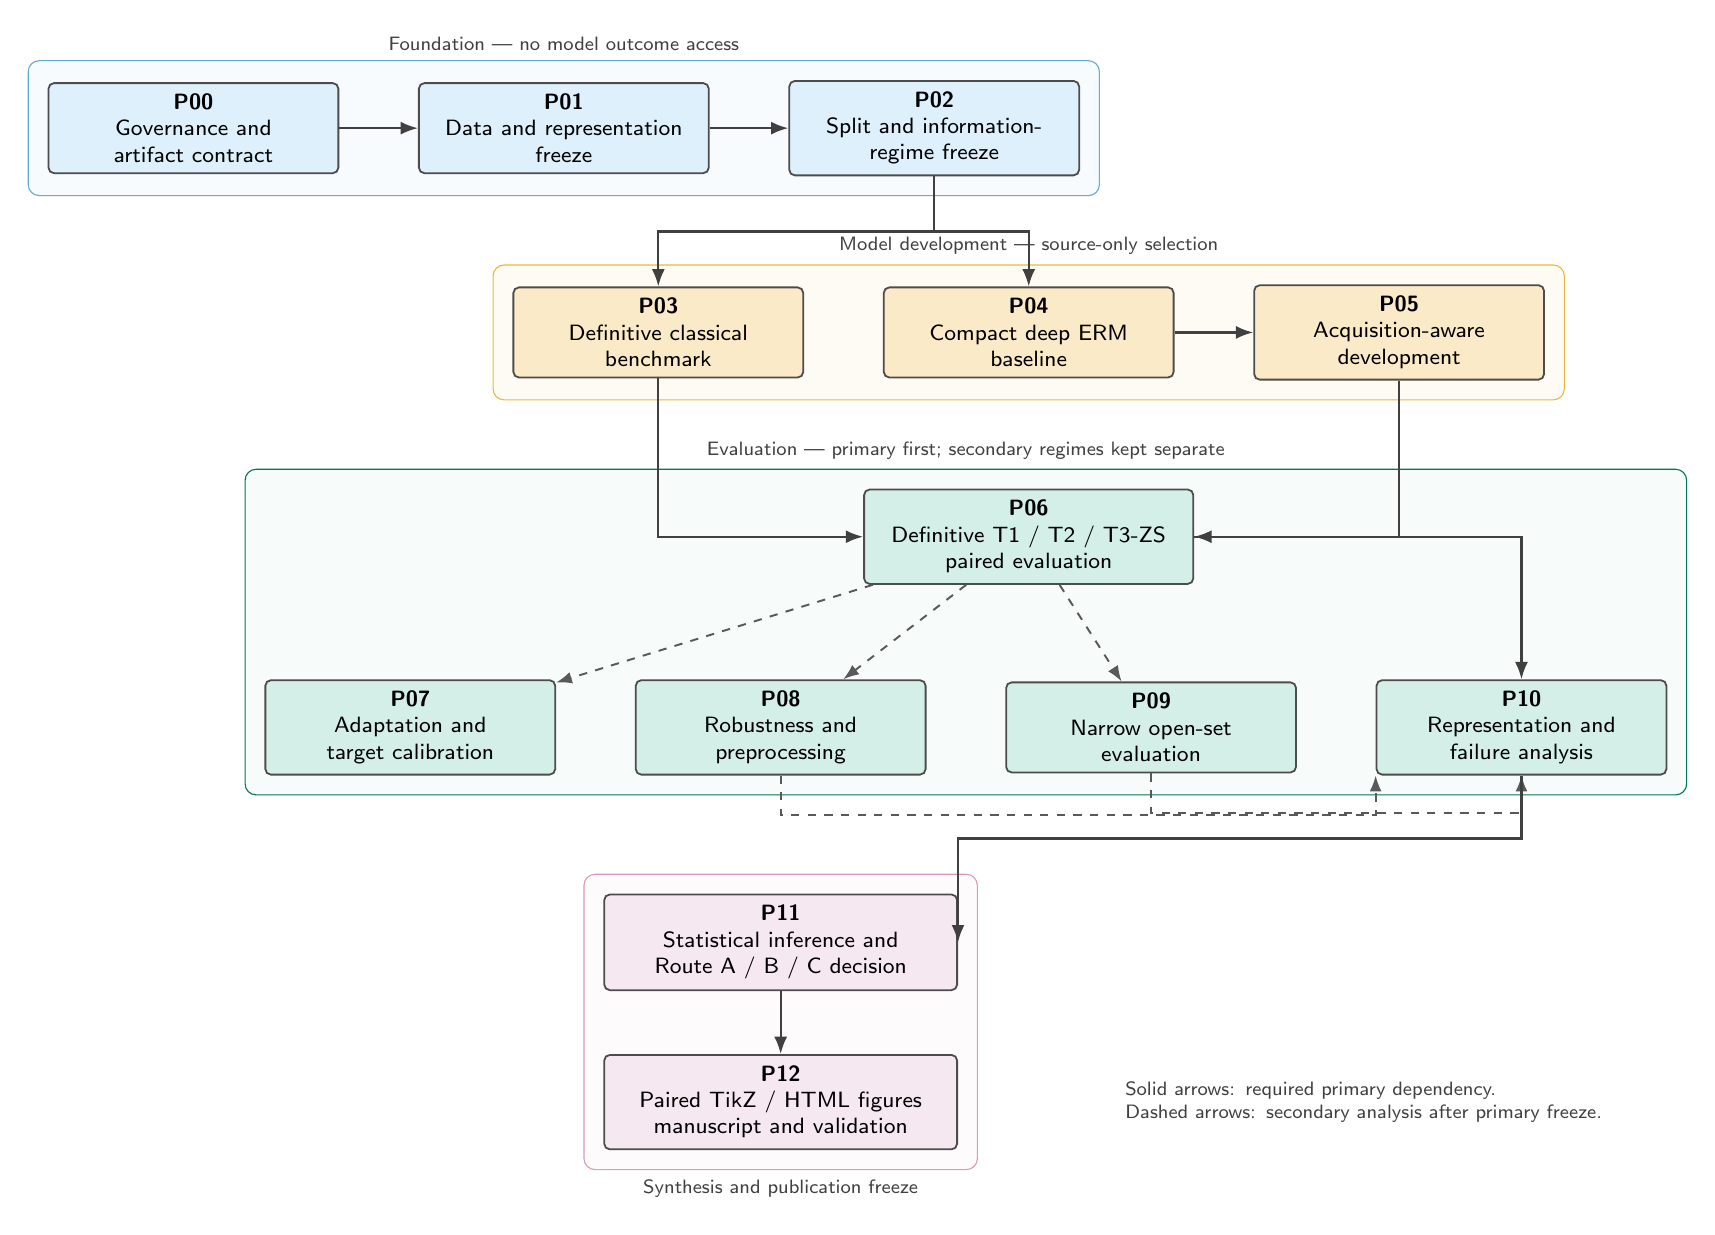
\begin{tikzpicture}[node distance=7mm and 10mm]
  \node[foundation] (p00) {\textbf{P00}\\Governance and\\artifact contract};
  \node[foundation, right=of p00] (p01) {\textbf{P01}\\Data and representation\\freeze};
  \node[foundation, right=of p01] (p02) {\textbf{P02}\\Split and information-\\regime freeze};

  \node[modeling, below left=14mm and -2mm of p02] (p03) {\textbf{P03}\\Definitive classical\\benchmark};
  \node[modeling, right=of p03] (p04) {\textbf{P04}\\Compact deep ERM\\baseline};
  \node[modeling, right=of p04] (p05) {\textbf{P05}\\Acquisition-aware\\development};

  \node[evaluation, below=14mm of p04, text width=39mm] (p06) {\textbf{P06}\\Definitive T1 / T2 / T3-ZS\\paired evaluation};
  \node[evaluation, below left=12mm and 39mm of p06] (p07) {\textbf{P07}\\Adaptation and\\target calibration};
  \node[evaluation, right=of p07] (p08) {\textbf{P08}\\Robustness and\\preprocessing};
  \node[evaluation, right=of p08] (p09) {\textbf{P09}\\Narrow open-set\\evaluation};
  \node[evaluation, right=of p09] (p10) {\textbf{P10}\\Representation and\\failure analysis};

  \node[synthesis, below=15mm of p08, text width=42mm] (p11) {\textbf{P11}\\Statistical inference and\\Route A / B / C decision};
  \node[synthesis, below=8mm of p11, text width=42mm] (p12) {\textbf{P12}\\Paired TikZ / HTML figures\\manuscript and validation};

  \draw[flow] (p00) -- (p01);
  \draw[flow] (p01) -- (p02);
  \draw[flow] (p02.south) -- ++(0,-7mm) -| (p03.north);
  \draw[flow] (p02.south) -- ++(0,-7mm) -| (p04.north);
  \draw[flow] (p04) -- (p05);
  \draw[flow] (p03.south) |- (p06.west);
  \draw[flow] (p05.south) |- (p06.east);
  \draw[secondaryflow] (p06) -- (p07);
  \draw[secondaryflow] (p06) -- (p08);
  \draw[secondaryflow] (p06) -- (p09);
  \draw[flow] (p06.east) -| (p10.north);
  \draw[secondaryflow] (p08.south) -- ++(0,-5mm) -| (p10.south west);
  \draw[secondaryflow] (p09.south) -- ++(0,-5mm) -| (p10.south);
  \draw[flow] (p10.south) -- ++(0,-8mm) -| (p11.east);
  \draw[flow] (p11) -- (p12);

  \begin{scope}[on background layer]
    \node[draw=oiBlue!60, rounded corners=4pt, fill=oiSky!5, fit=(p00)(p01)(p02),
      inner sep=7pt, label={[labeltext]above:Foundation --- no model outcome access}] {};
    \node[draw=oiOrange!75, rounded corners=4pt, fill=oiOrange!4, fit=(p03)(p04)(p05),
      inner sep=7pt, label={[labeltext]above:Model development --- source-only selection}] {};
    \node[draw=oiGreen!75!black, rounded corners=4pt, fill=oiGreen!3, fit=(p06)(p07)(p08)(p09)(p10),
      inner sep=7pt, label={[labeltext]above:Evaluation --- primary first; secondary regimes kept separate}] {};
    \node[draw=oiPurple!75, rounded corners=4pt, fill=oiPurple!3, fit=(p11)(p12),
      inner sep=7pt, label={[labeltext]below:Synthesis and publication freeze}] {};
  \end{scope}

  \node[labeltext, right=20mm of p12, align=left, text width=63mm] {Solid arrows: required primary dependency.\\Dashed arrows: secondary analysis after primary freeze.};
\end{tikzpicture}
\end{document}
